%\documentclass[10pt,t]{beamer}
%
\documentclass[10pt,t,handout]{beamer}
\usetheme{Heverlee}
\usepackage[UTF8]{ctex}
%\usepackage{CJKutf8}
\usepackage{hyperref}
\graphicspath{{imags/}}
\newcommand{\tr}{\textcolor{red}}
\newcommand{\tc}{\textcolor{cyan}}
\newcommand{\tb}{\textcolor{blue}}
\newcommand{\ty}{\textcolor{yellow}}
\newcommand{\bc}{\colorbox{cyan}}
\usepackage{xcolor}
\usepackage{graphicx}
\usepackage{multicol}
 
    \logo{
\includegraphics[height=0.7cm]{logo1.png}\hspace{4pt}\vspace{-6pt}}

\AtBeginSection[]
{
	\begin{frame}<beamer>
		\frametitle{\textbf{目录}}
		\tableofcontents[currentsection]
	\end{frame}
}
\beamerdefaultoverlayspecification{<+->}

%%% TITLE PAGE INFO:
\title{Transformer在时间序列中的应用}
\author{刁姝心、沙漠、陆佳欢}
\institute{数学科学学院  }
\date{2022.4.13}
\begin{document}
{
\usebackgroundtemplate{ \parbox[b][\paperheight][b]{\paperwidth}{\centering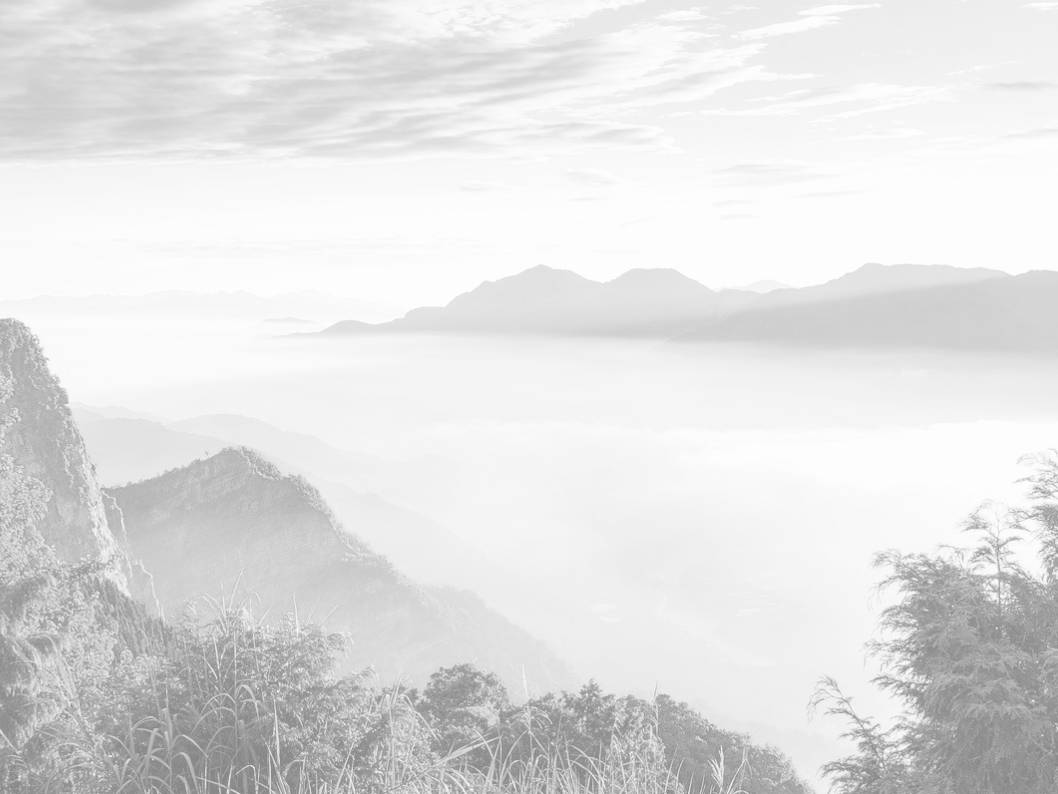
\includegraphics[width=\paperwidth]{Background/bg_alishan.jpg}}}

\begin{frame}[plain,noframenumbering]
    \titlepage
\end{frame}
}		
\begin{frame}
	
	\
	
	\
	
	{\color{red}{\large\textbf{基本信息}} }
	
	\

	{\color{blue}{\textbf{刁姝心}} }
	
	\
	
	Email: 1446107067@qq.com~~~~~~~~~~~~~~	Tel: 18252587369
	\
	
	QQ: 1446107067~~~~~~~~~~~~~~~~~~~~~~~~~~~~~~ 
	
	\
	
	\
	
	
	{\color{blue}{\textbf{沙漠}} }
	
	\
	
	Email: 2300024266@qq.com~~~~~~~~~~~~~~	Tel: 18052526508
		\
	
	QQ: 2300024266~~~~~~~~~~~~~~~~~~~~~~~~~~~~~~ 
	
\

\

	{\color{blue}{\textbf{陆佳欢}} }

\

Email: 207829897@qq.com~~~~~~~~~~~~~~	Tel: 17849061238
\

QQ: 207829897~~~~~~~~~~~~~~~~~~~~~~~~~~~~~~ 

\

\

\end{frame}

   %目录
\begin{frame}{目录}
	\tableofcontents
\end{frame}
\section{引言} 
 \begin{frame} 
\frametitle{统计学对时间序列的研究} 
  	\begin{figure}
  	\centering
  	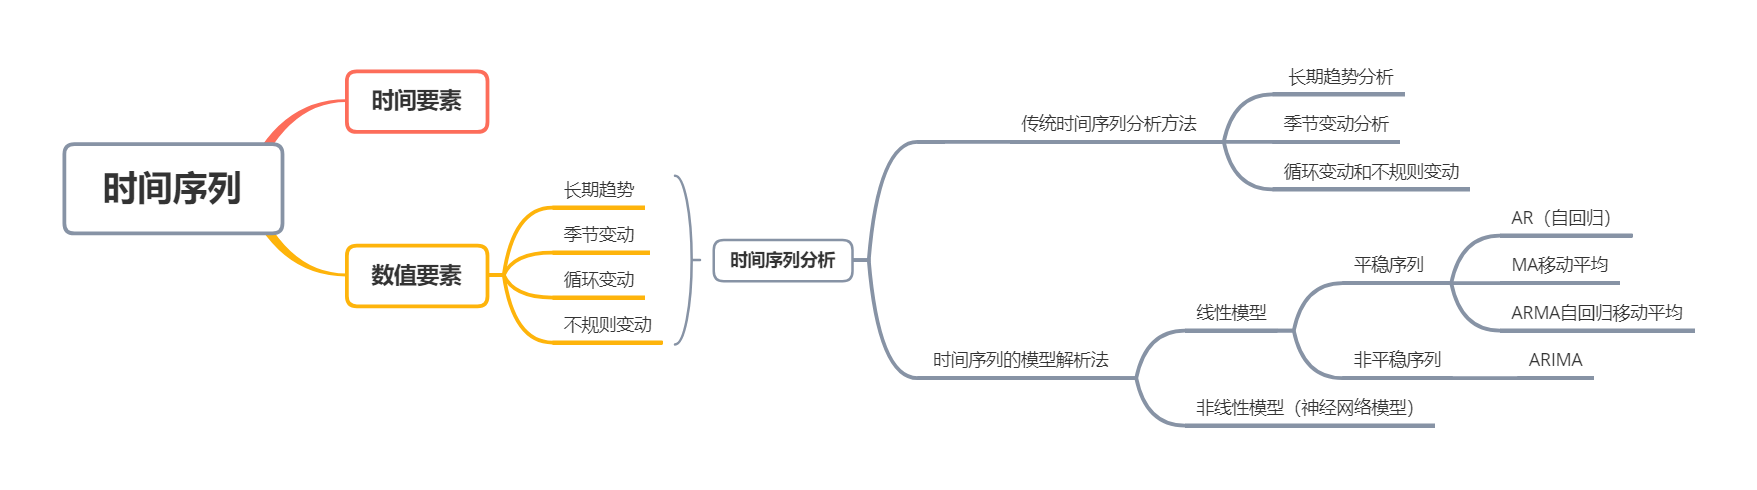
\includegraphics[width=11cm,height=4.5cm]{时间序列.png}	
  	%	\caption{统计学时间序列分析}
  	\label{fig:caps}
  \end{figure}
 \end{frame}
\begin{frame}
\frametitle{时间序列在深度学习上的体现} 
\begin{figure}
	\begin{columns}[T] % align columns
		\begin{column}<0->{.45\textwidth}
			\begin{figure}[thpb]
				\centering
				\resizebox{1\linewidth}{!}{
					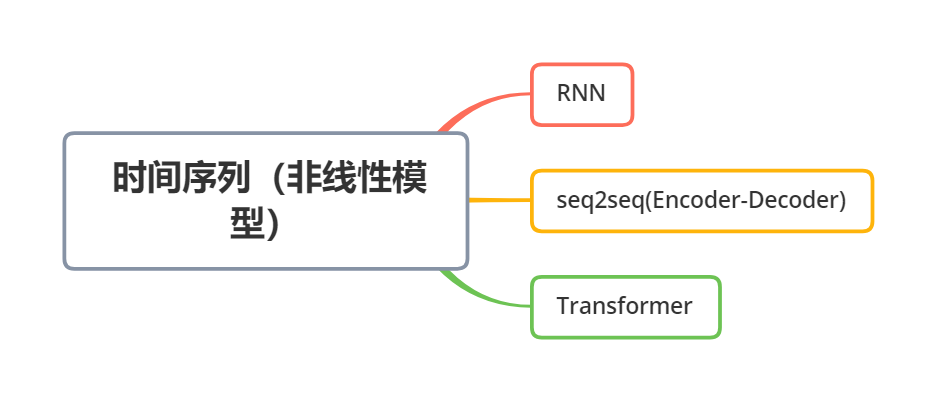
\includegraphics{2.png}
				}
				%\includegraphics[scale=1.0]{figurefile}
				\caption{序列模型方法}
				\label{fig:camps}
			\end{figure}
			\begin{figure}[thpb]
			\centering
			\resizebox{1\linewidth}{!}{
				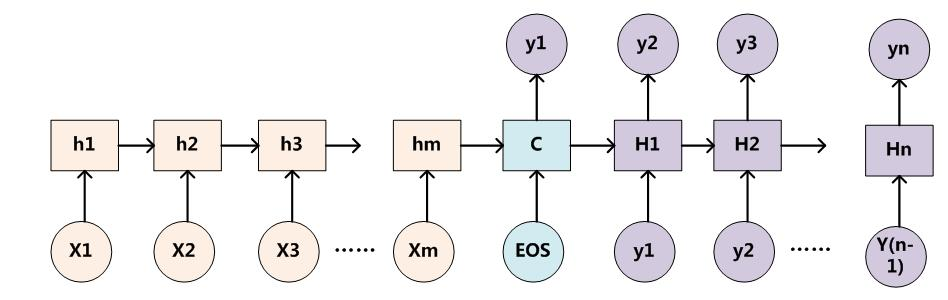
\includegraphics{im.png}
			}
			%\includegraphics[scale=1.0]{figurefile}
			\caption{RNN Encoder-Decoder 框架}
			\label{fig:mps}
		\end{figure}
		\end{column}%
		\hfill%
		\begin{column}<0->{.6\textwidth}
			\begin{itemize}
				\item<1-> RNN由于其顺序性以及时间平移非对称的特性,通常模型会更容易受到输入序列中较后位置的数据的影响。
				
				\
				
				\item<2->  seq2seq是标准的Enocder-Decoder模型,加入attention后从而能够保存更多的信息。
				
				\
				
				\item<3-> Transfromer不必顺序翻译文本,提高模型的并行能力,解决LSTM无法缓解的长期依赖问题。
			 
			\end{itemize}
		\end{column}%
	\end{columns}
\end{figure}
\end{frame}
\section{Transformer的原理}  
\begin{frame}
\frametitle{Transformer架构}
\begin{figure}
	\centering
	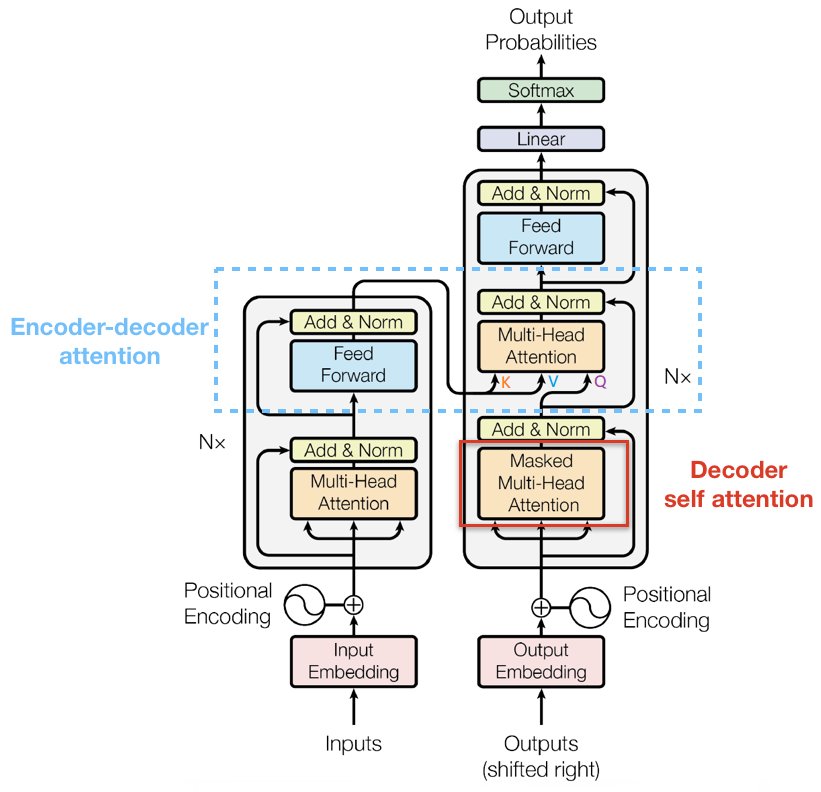
\includegraphics[width=7.5cm]{transformer架构.png}
\end{figure}
\end{frame}
\begin{frame}
\frametitle{Transformer结构}
\begin{figure}
	\begin{columns}[T] % align columns
		\begin{column}<0->{.45\textwidth}
			\begin{figure}[thpb]
				\centering
				\resizebox{1\linewidth}{!}{
					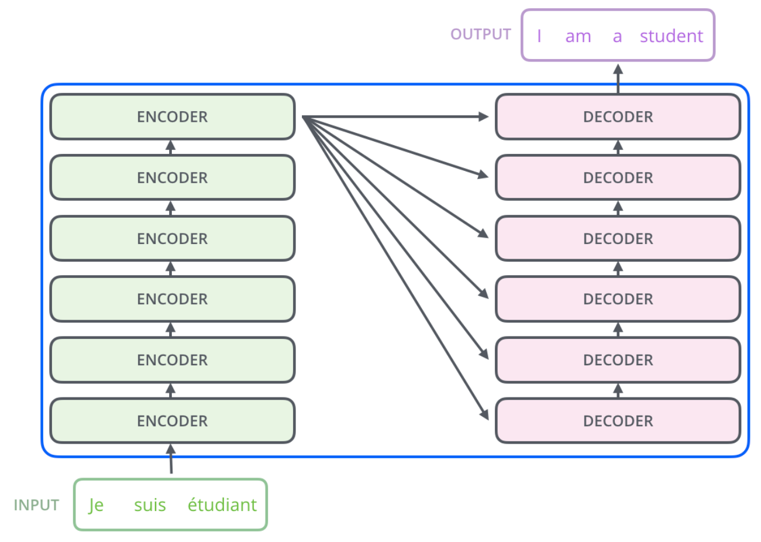
\includegraphics{3.png}
				}
				%\includegraphics[scale=1.0]{figurefile}
				\caption{Transformer整体结构}
				\label{fig:m}
			\end{figure}
			\begin{figure}[thpb]
				\centering
				\resizebox{1\linewidth}{!}{
					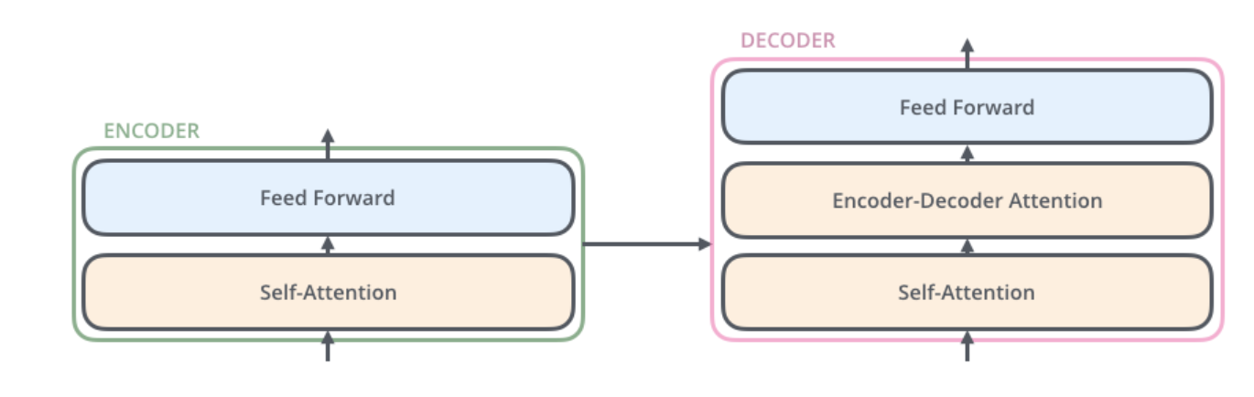
\includegraphics{4.png}
				}
				%\includegraphics[scale=1.0]{figurefile}
				\caption{encoder-decoder}
				\label{fimps}
			\end{figure}
		\end{column}
		\hfill
		\begin{column}<0->{.5\textwidth}
			\begin{itemize}
			 
				\item<1->  编码部分(6个编码器)
				
				\
				\item<2->	解码部分(6个解码器)
				
				\
				
				\
				
				\
				
				\item<3->  编码器(自注意力 + FFN) 
				
				\
				\item<4->解码器(自注意力 + 掩码注意力 + FFN)
			 
				
			\end{itemize}
		\end{column}%
	\end{columns}
\end{figure}
\end{frame}
\begin{frame}
\frametitle{Positional Encoding}
Transformer抛弃了RNN,而RNN最大的优点就是在时间序列上对数据的抽象,所以文章中作者提出两种Positional Encoding的方法,将encoding后的数据与embedding数据求和,加入了相对位置信息。
\begin{block}{\textbf{基本思路}}
	\begin{enumerate}
		\item<0->  用不同频率的sine和cosine函数直接计算 
		\item<0-> 学习出一份positional embedding
	\end{enumerate}
\
\
实验发现两种效果一样,作者选择了第一种。
\end{block}
	\begin{figure}
	\centering
	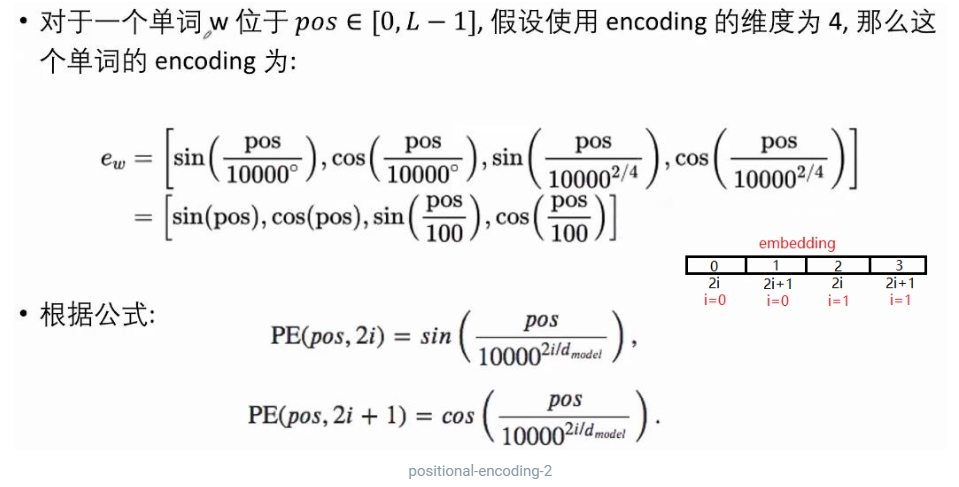
\includegraphics[scale=.3]{14.png}	~~~~
	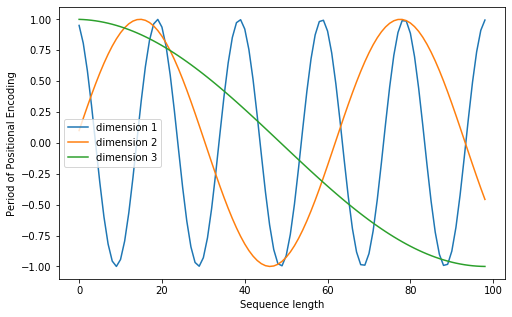
\includegraphics[scale=.2]{15.png}  ~~~~
%	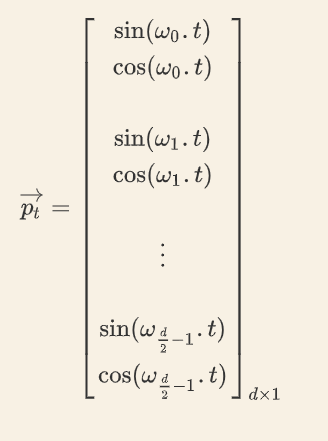
\includegraphics[scale=.1]{16.png}
\end{figure}

\end{frame}
\begin{frame}
\frametitle{self-attention}

       \
       
	{\color{red}{\large\textbf{向量计算}} }
	\
	
	\
		\begin{columns}[T] % align columns
		\begin{column}<0->{.45\textwidth}
			\begin{figure}[thpb]
				\centering
				\resizebox{1\linewidth}{!}{
					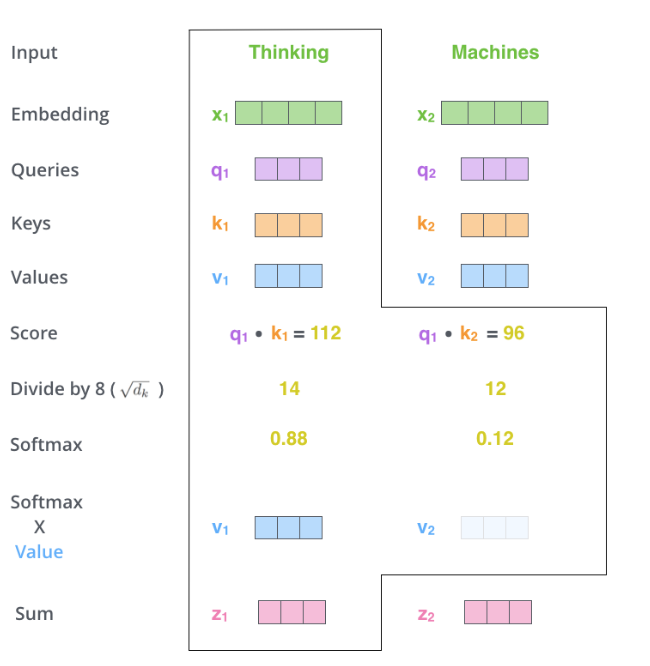
\includegraphics{5.png}
				}
				%\includegraphics[scale=1.0]{figurefile}
			 
				\label{f:m}
			\end{figure}
		\end{column}
		\hfill
	\begin{column}<0->{.5\textwidth}
	 	\begin{itemize}
	 		\item<1->  计算$q_1$,$k_1$,$v_1$.\\
	 	\begin{figure}[thpb]
	 	
	 	\resizebox{1\linewidth}{!}{
	 		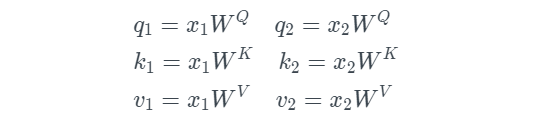
\includegraphics{11.png}
	 	}
	 	%\includegraphics[scale=1.0]{figurefile}
	 	
	 	\label{f1:m}
	 \end{figure}
 	\item<1->   求权重$\theta $.\\
 	\begin{figure}[thpb]
 		
 		\resizebox{1\linewidth}{!}{
 			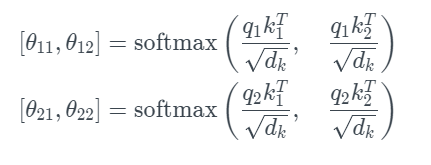
\includegraphics{12.png}
 		}
 		%\includegraphics[scale=1.0]{figurefile}
 		
 		\label{f112m}
 	\end{figure}
 	\item<3->   求$z_1$,$z_2$\\
 		\begin{figure}[thpb]
 		
 		\resizebox{1\linewidth}{!}{
 			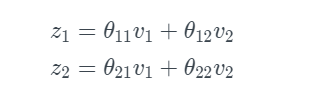
\includegraphics{13.png}
 		}
 		%\includegraphics[scale=1.0]{figurefile}
 		
 		\label{f11as2m}
 	\end{figure}
 	\end{itemize}
	\end{column}
\end{columns}
 
\end{frame}
\begin{frame}

\

{\color{red}{\large\textbf{矩阵计算}} }
\

\
\
	\begin{itemize}
	\item<1-> 词嵌入的矩阵$X$乘以训练的权值矩阵($W^{Q}$,$W^{K}$,$W^{V}$)
	
	\ 
	\begin{figure}[!t]
		\centering
		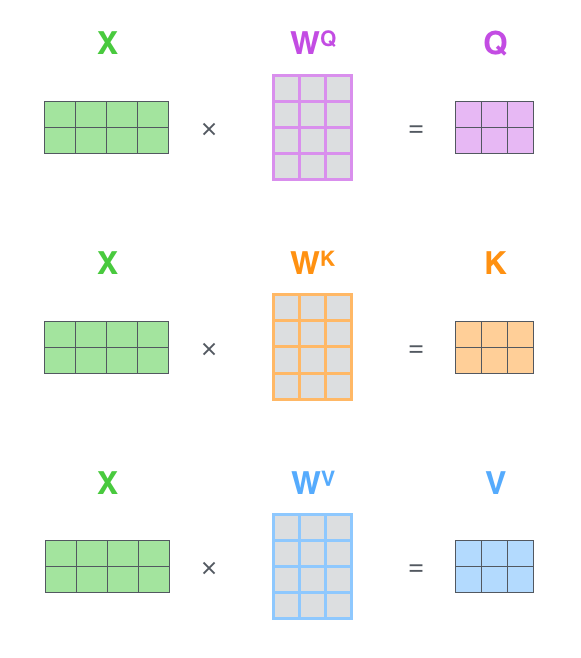
\includegraphics[scale=0.12]{111.png}
		\label{figure3_OT}
	\end{figure}
\

	\item<2-> 使用$\operatorname{Attention}(Q, K, V)=\operatorname{softmax}\left(\frac{Q K^{T}}{\sqrt{d_{k}}}\right) V$.计算$Z$
	\
	
	\
		\begin{figure}[!t]
		\centering
		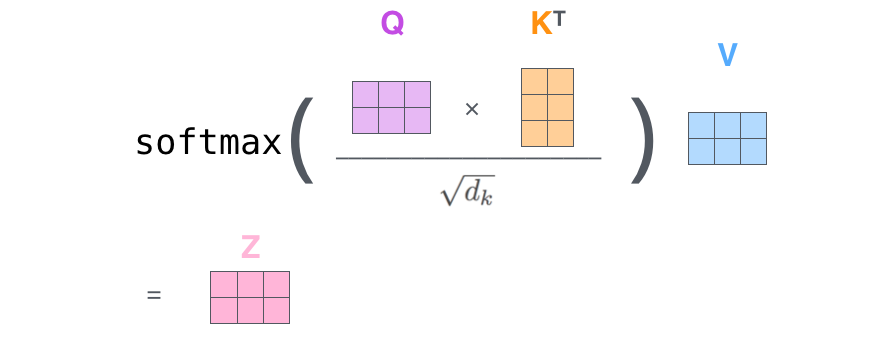
\includegraphics[scale=0.14]{1111.png}
		\label{figurOT}
	\end{figure}
	\end{itemize}
\end{frame}
\begin{frame}
	\frametitle{Multi-head self-attention}
 	\begin{figure}
 	\centering
 	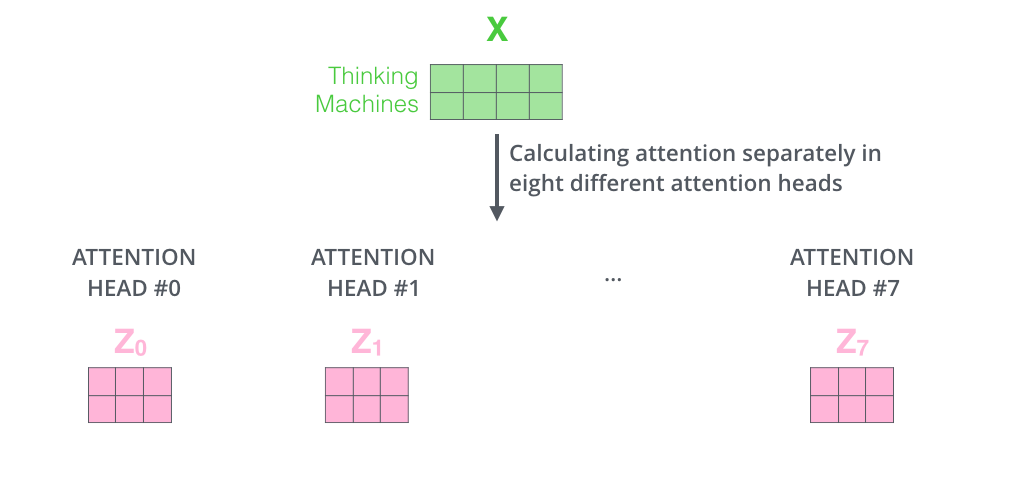
\includegraphics[width=5cm]{222.png}	~~~~
 	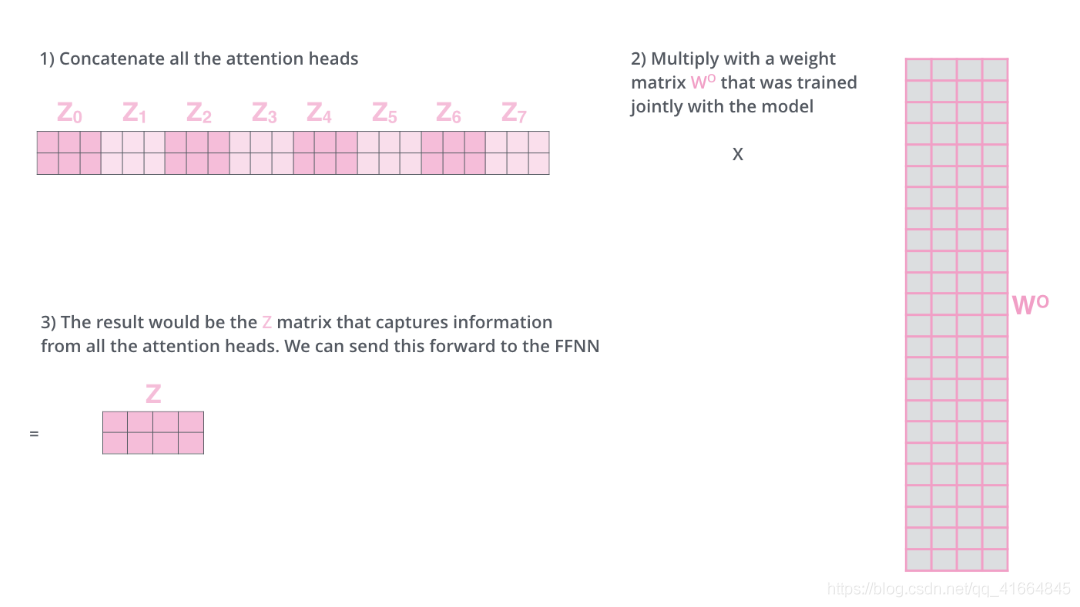
\includegraphics[width=5cm]{333.png}	
 \end{figure}
\begin{itemize}

	\item<1-> 使用多组$W^{Q}, W^{K}, W^{V}$,以此来关注不同上下文,求特征矩阵$Z_{i}$
	\
	
	\
 
	\item<2->  将$Z_{i}$按列拼接成一个大特征矩阵并通过一层全连接层得到输出$Z$.
\end{itemize}
\begin{figure}
		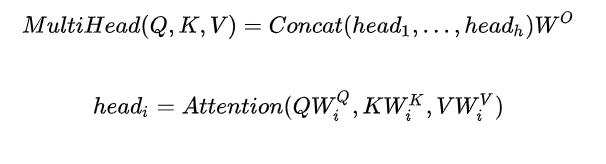
\includegraphics[width=7cm]{9.png}	
\end{figure}
\end{frame}

\begin{frame}

\frametitle{skip connection \& Layer Normalization}

$Add \& Norm$ 模块$\rightarrow $LayerNorm $(x+\operatorname{Sublayer}(x))$
 
 \begin{block}{\textbf{残差连接}}
 	\begin{itemize}
 		\item<0-> self-attention 加权之后输出,也就是Self-Attention $(Q, K, V)$ ,然后把他们加起来做残差连接。
 		$$
 		X_{\text {embedding }}+\text { MultiHeadAttention }(Q, K, V)
 		$$  
 	\end{itemize}
 \end{block}
 
  \begin{block}{\textbf{LN}}
 	\begin{itemize}
 		\item<0-> BN它是取不同样本的同一个通道的特征做归一化;LN它取的是同一个样本的不同通道做归一化。
 	 $$
 	 \operatorname{Layer} \operatorname{Norm}(x)=\frac{x_{i j}-\mu_{j}}{\sqrt{\sigma_{j}^{2}+\epsilon}}
 	 $$
 	\end{itemize}
 \end{block}
\end{frame}
\begin{frame}
\frametitle{FFN}
 \begin{block}{\textbf{FFN}}
	\begin{itemize}
		\item<0-> FFN即Feed Forward Neural Network。这个全连接有两层,第一层的激活函数是ReLU,第二层是一个线性激活函数,可以表示为:
	 $$
	 \operatorname{FFN}(Z)=\max \left(0, Z W_{1}+b_{1}\right) W_{2}+b_{2}
	 $$
	 	\item<0->若选择ReLU则,当做完残差和LN后得到X特征矩阵然后再做如下操作:\\
	 	$$
	 	X_{\text {hidden }}=\operatorname{Linear}\left(\operatorname{ReLU}\left(\text { Linear }\left(X_{a t t e n t i o n}\right)\right)\right)
	 	$$ 
	 	$$
	 	X_{\text {hidden }}=X_{\text {attention }}+X_{\text {hidden }}
	 	$$
	 	$$
	 	X_{h i d d e n}=\operatorname{LayerNorm}\left(X_{\text {hidden }}\right)
	 	$$ 
	 	其中$X_{\text {attention }}$是残差层的结果。
	\end{itemize}
\end{block}
Encoder block 接收输入矩阵$X_{nxd}$,输出一个矩阵$O_{nxd}$.最后一个block 输出的矩阵就是编码信息矩阵 C,这一矩阵后续会用到 Decoder 中。
\end{frame}
\begin{frame}
\frametitle{Masked Self-Attention}
Seq2Seq 中 Decoder 使用的是 RNN 模型,由于循环神经网络是时间驱动的,只有当  时刻运算结束了,才能看到  时刻的词。而 Transformer Decoder 抛弃了 RNN,改为 Self-Attention,由此就产生了一个问题,在训练过程中,整个 ground truth 都暴露在 Decoder 中,这显然是不对的,我们需要对 Decoder 的输入进行一些处理,该处理被称为 Mask.

\

\
\begin{figure}
  	\centering
  	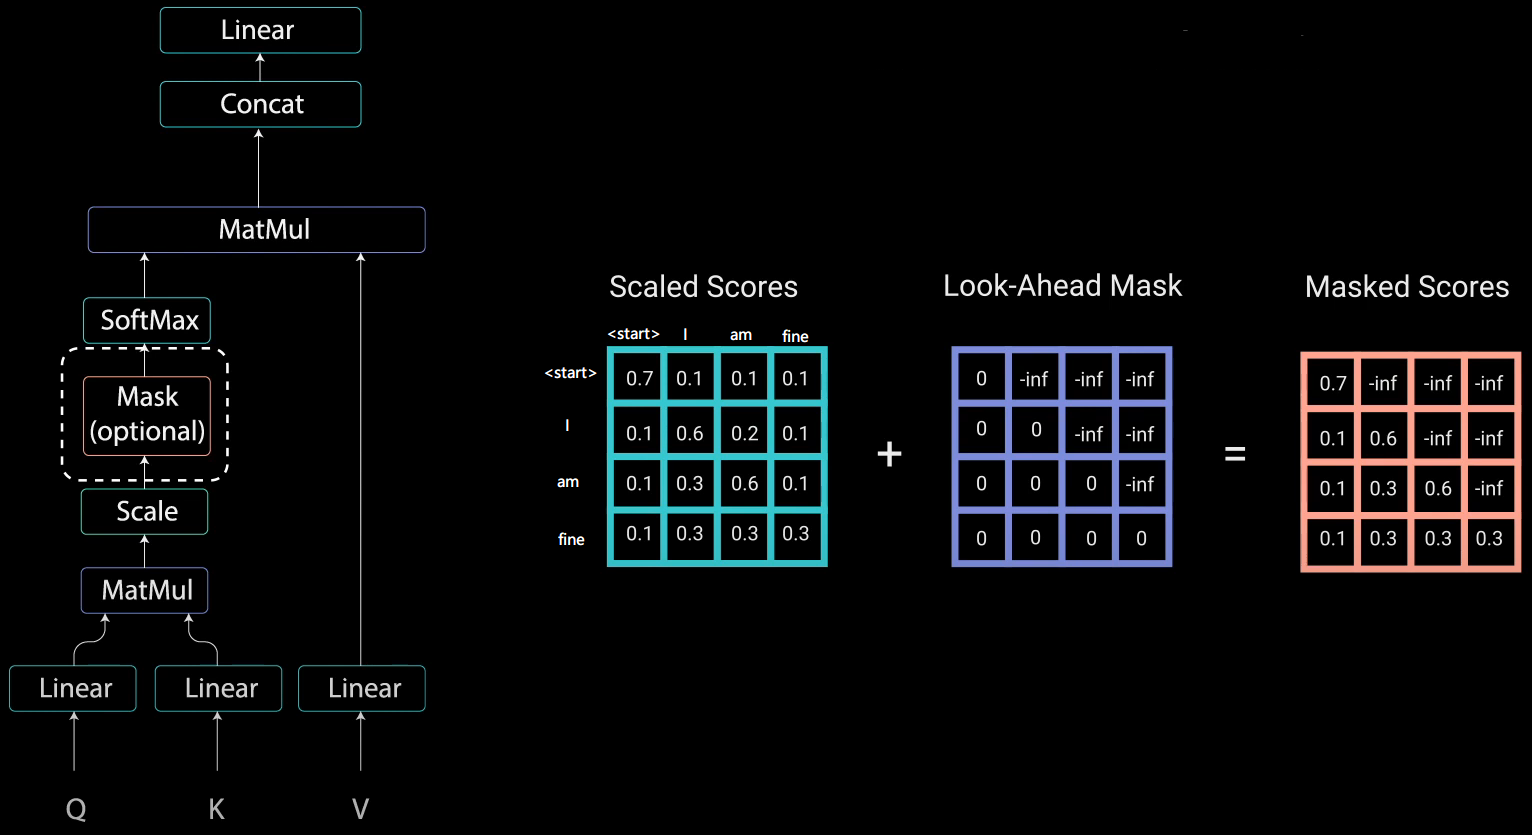
\includegraphics[width=5.5cm]{ 111111.png}	~~~~
  	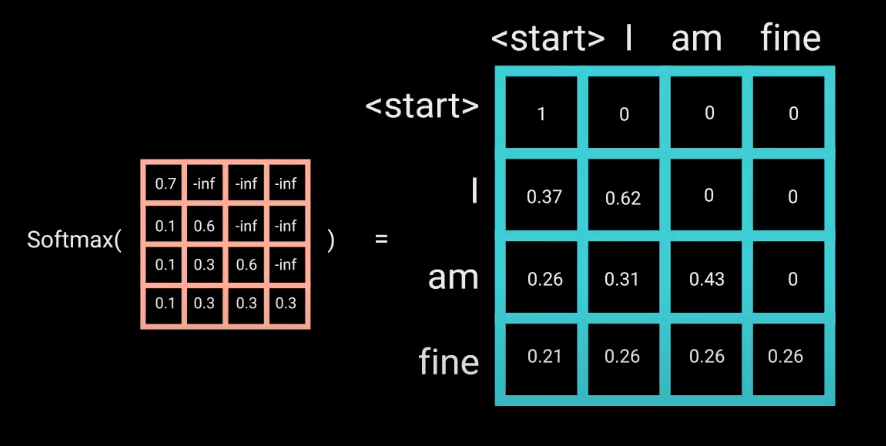
\includegraphics[width=4.5cm]{0.png}	
 	\caption{Mask $QK^T$}
  
\end{figure}

\end{frame}
\begin{frame}

\

\

{\color{red}{\large\textbf{流程如下:}} }

\

\
\begin{block}{\textbf{Masked Self-attention步骤}}
	\begin{enumerate}
		\item<0-> 对于Decoder 的输入矩阵和 Mask 矩阵,输入矩阵包含所有单词(翻译完)的表示向量,Mask与输入矩阵同维且遮挡X的某些单词信息。在 Mask矩阵中,前面的单词只能用前面的信息。
		\
		\
		\item<0-> 接下来的操作和之前的 Self-Attention 一样,通过输入矩阵 X 计算得到 Q, K, V 矩阵。然后计算 Q 和 $K^{T}$ 的乘积 $QK^T$。
		\
		\
		\item<0-> 在得到 $QK^{T}$ 之后需要进行 Softmax,计算 attention score,我们在 Softmax 之前需要使用 Mask 矩阵遮挡住每一个单词之后的信息 。得到  $QK^{T}$之后在  $QK^{T}$ 上进行 Softmax,每一行的和都为 1。但是单词 0 在单词 1, 2, 3, 4 上的 attention score 都为 0。
		\item<0-> 使用 Mask $QK^T$ 与矩阵 V 相乘,得到输出 Z,则Z中前面的单词只包含前面的信息。
	 
	\end{enumerate}
\end{block}
\end{frame}
\begin{frame}
\frametitle{Masked Encoder-Decoder Attention}
	\begin{figure}
		\begin{columns}[T] % align columns
			\begin{column}<0->{.55\textwidth}
				\begin{figure}[thpb]
					\centering
					\resizebox{1\linewidth}{!}{
						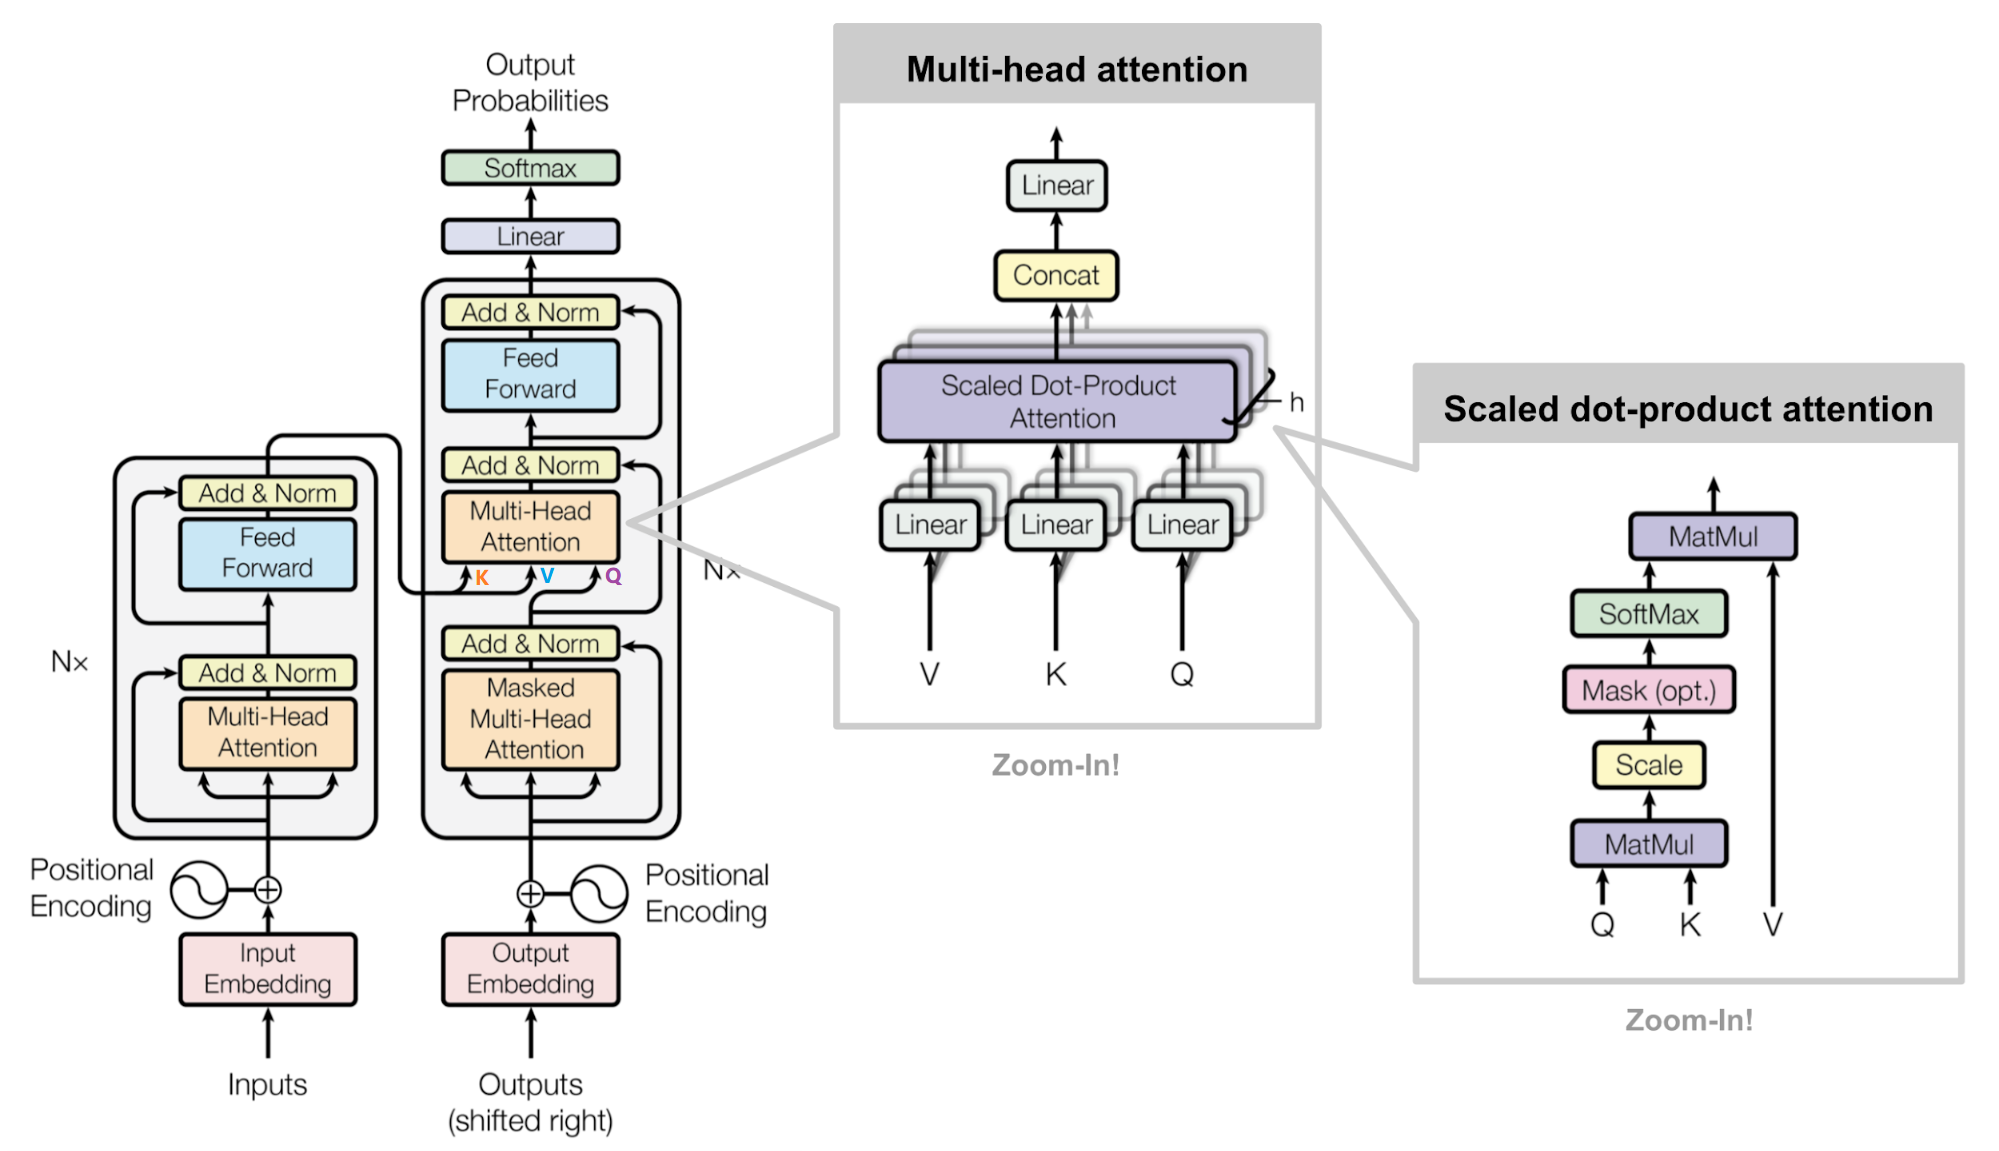
\includegraphics{50.png}
					}
					%\includegraphics[scale=1.0]{figurefile}
					\caption{序列模型方法}
					\label{fmps}
				\end{figure}
				 
			\end{column}%
			\hfill%
			\begin{column}<0->{.45\textwidth}
				\begin{itemize}
					\item<1-> K, V 矩阵不是使用 上一个 Decoder block 的输出计算的,而是使用 Encoder 的编码信息矩阵 C 计算的。
					
					\
					
					\item<2->  根据 Encoder 的输出 C 计算得到 K, V,根据上一个 Decoder block 的输出 Z 计算 Q (如果是第一个 Decoder block 则使用输入矩阵 X 进行计算) 
					 
					\
					
					\item<3-> Transfromer不必顺序翻译文本,提高模型的并行能力,解决LSTM无法缓解的长期依赖问题。
					
				\end{itemize}
			\end{column}%
		\end{columns}
	\end{figure}
\end{frame}
\section{时间序列的Transformer模型}
 \begin{frame}
 \frametitle{时间序列Transformer模型}	
  	\begin{figure}
  	\centering
  	\includegraphics[scale=0.4]{图.png}	~~~~
 
  \end{figure}
  
 \end{frame}
\begin{frame}

\

\

{\color{red}{\large\textbf{时间序列的网络化}} }

\
 
	\begin{itemize}
		\item<1-> Positional Encoding
		\begin{itemize}
			\item<1-> 原始的位置编码送入Transformer,不能充分利用时间序列数据信息,也不能适应不同的数据。 
			\item<1-> Learnable Positional Encoding通过学习每个位置的一组位置嵌入能表征更丰富的位置信息,这样学习到的位置嵌入更灵活,能够适应特定的任务。
			\item<1->Timestamp Encoding通常可以获得时间戳信息 但在Transformer中几乎没有得到利用。 
			
		\end{itemize}
		\item<2-> Attention Module
		\begin{itemize}
			\item<2-> 
原始Transformer的时间和内存复杂度是$O(L^2)$其中$L$是输入序列长度,许多模型尝试减少这一计算复度,主要依赖稀疏性或者低秩近似的方式。
		\end{itemize}
		\item<3-> Architecture-Level Innovation
	\begin{itemize}
		\item<3-> 可以以较低的计算复杂度处理较长序列;

		\item<3-> 层次建模可以获得多分辨率表示,对特定任务是有用的。 
		
	\end{itemize}
	\end{itemize}

\end{frame}
 \begin{frame}
 	
 	\
 	
 	\
 	
 	{\color{red}{\large\textbf{时间序列Transformer应用场景}} }
 	
 	\
 		\begin{figure}
 		\centering
 		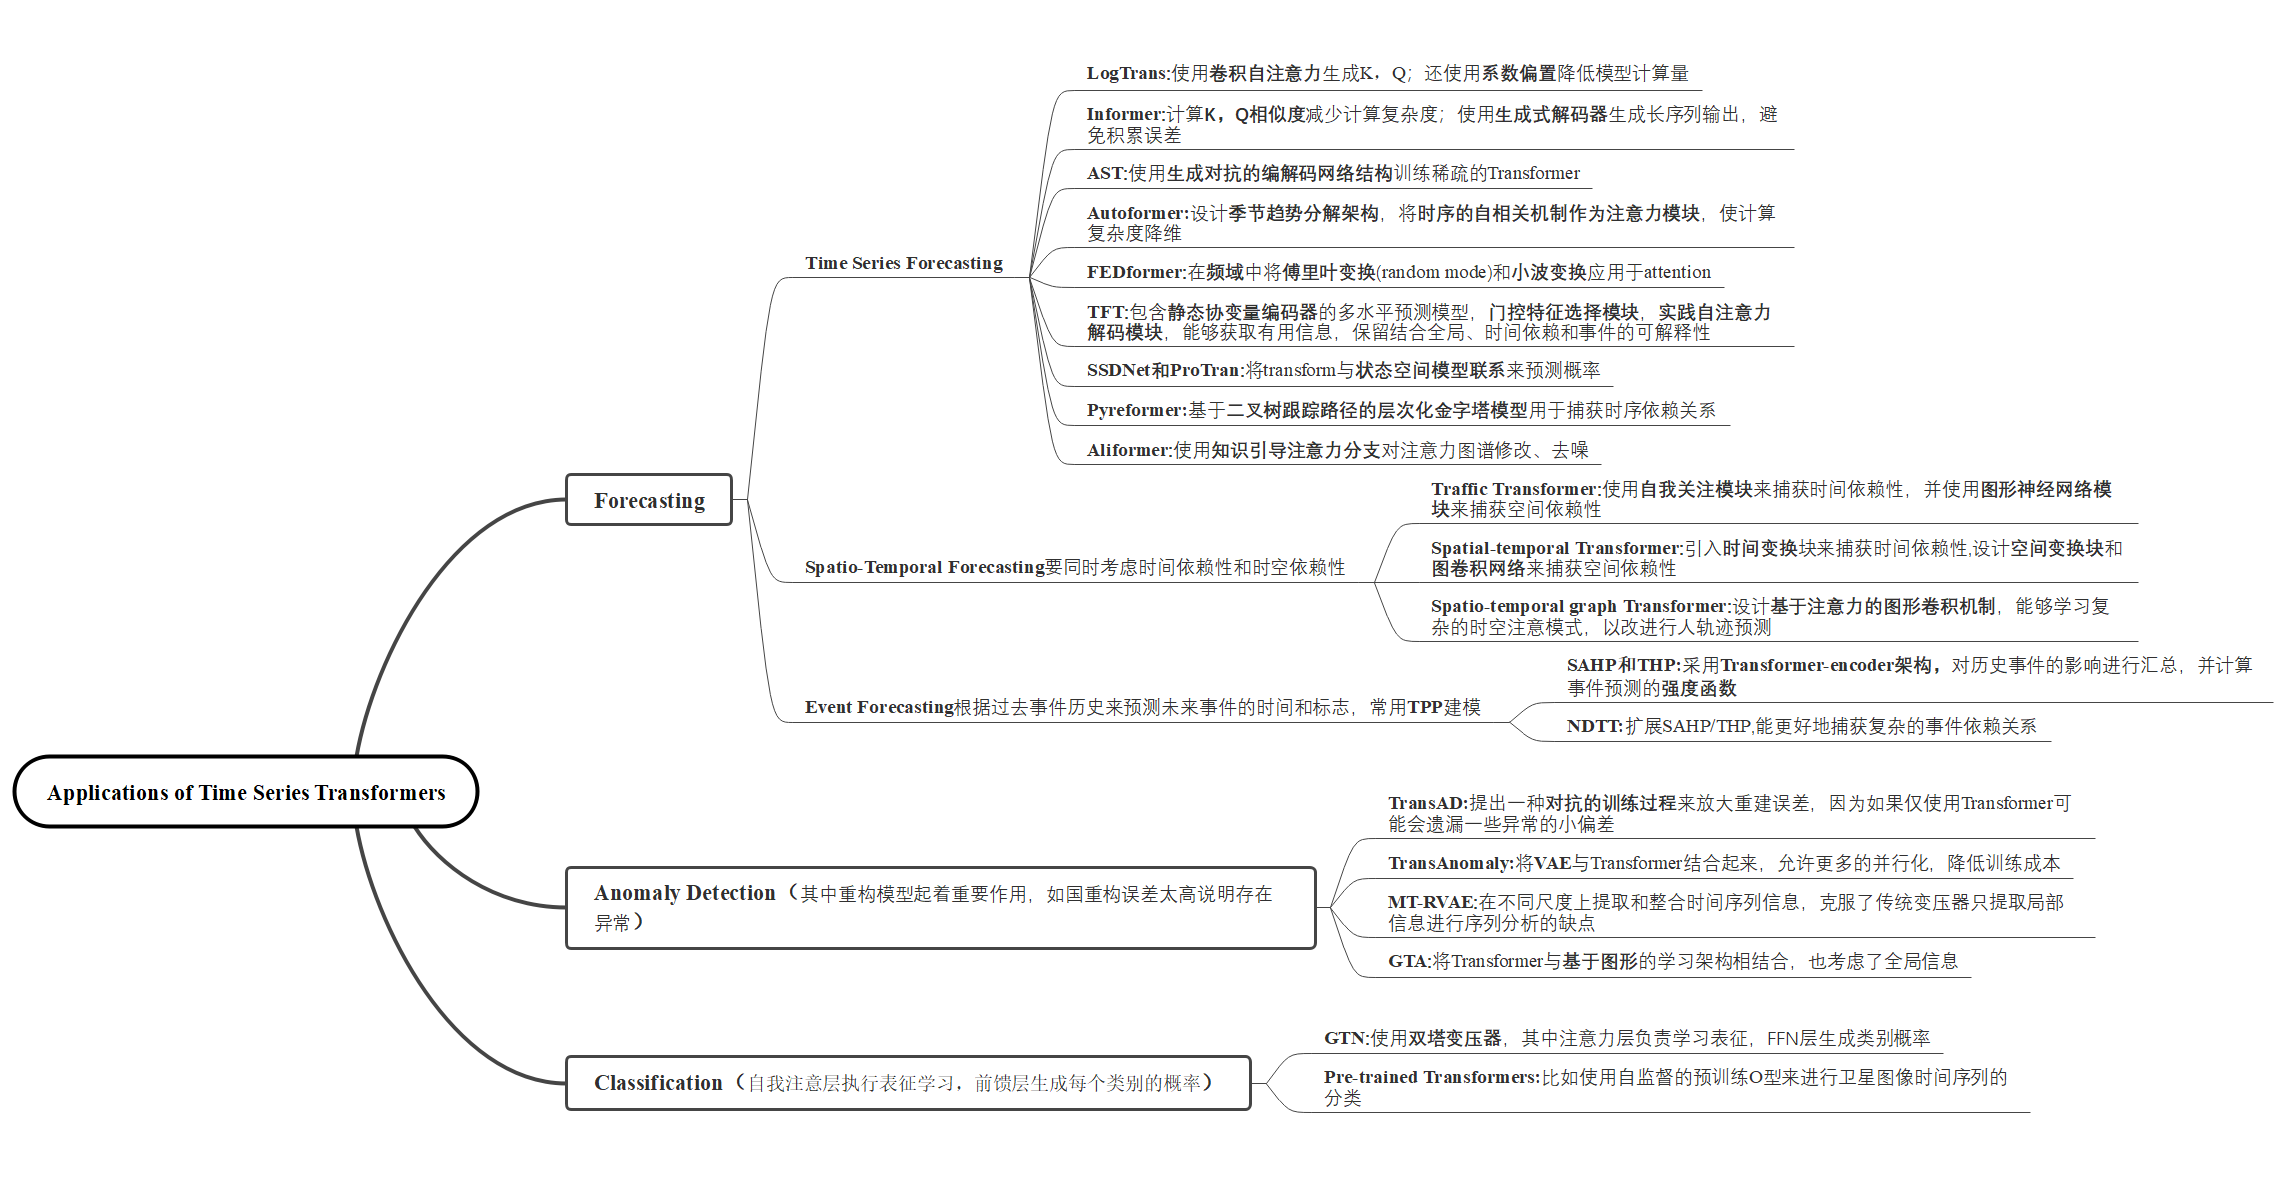
\includegraphics[scale=0.41]{应用.png}	~~~~
 		
 	\end{figure}
 	
 \end{frame}
\section{实验评估与讨论}
\begin{frame}
\frametitle{实验评估与讨论}

\begin{itemize}
	\item<1->  鲁棒性分析
	\begin{itemize}
		\item<1-> "降低注意力计算复杂度一般使用小规模的输入"为了质疑这种观点而做了鲁棒性检验, 
		\item<1->  当输入序列长度变化是许多算法性能会迅速恶化,这种现象使得许多精心设计的Transformer模型在长序列的实际应用中不切实际,因为他们不能有效的利用长序列输入信息,需要进行更多的研究来充分适应长输入序列。	
	\end{itemize}

 	\
	\item<2->模型大小分析
	
	\begin{itemize}
		\item<2-> 3-6层的浅层次Transformer获得了最优结果,同时也提出一个问题,即如何设定一个合适的深度来提高模型的容量、获得最好的预测性能。

	\end{itemize}

\
	\item<3->season-trend分解分析
	\begin{itemize}
		\item<3-> seasonal-trend decomposition模块可以大幅度提升算法性能,提升高达50\%-80\%,这一独特的模块值得进一步研究。
 
		
	\end{itemize}
\end{itemize}
\end{frame}
\section{Future Work}	
\begin{frame} 
\frametitle{Future Work}
\begin{itemize}
	\item<1->  引入先验知识
	\begin{itemize}
		\item<1->将序列的周期性或者频域特点加入Transformer结构可以带来性能提升。
		\item<1-> 对特定时间序列和任务特点进行分析,采用最有效的方式引入先验知识,从而获得更优的Transformer架构。
	\end{itemize}
	
	\
	\item<2->引入GNN
	
	\begin{itemize}
		\item<2->引入图神经网络GNN是一种建模空间依赖性和维度间关系的方式。
		\item<2->
GNN与Transformer结合可以显著提升性能,还可以进行多模态预测、深入了解动态失控特征,因此二者的结合指的进一步研究。
	\end{itemize}
	
	\
	\item<3-> 预训练模型
	\begin{itemize}
		\item<3-> Transformer用于NLP需要大规模的预训练,但是对于时间序列的预训练Transformer模型研究有限,主要集中在时间序列的分类上,仍有很大的研究空间。
	\end{itemize}

\
\item<4->NAS设计模型
\begin{itemize}
	\item<4-> NAS可以有效解放人工,因此如何利用NAS自动设计高效的时间序列Transformer是值得研究的。
 
\end{itemize}

\end{itemize}
\end{frame}
 \begin{frame} 
 	\vspace*{\fill}
 	\begin{center}
 			\begin{center}
 			\begin{minipage}{1\textwidth}
 				
 				\setbeamercolor{mybox}{fg=white, bg=black!50!blue}
 				\begin{beamercolorbox}[wd=0.70\textwidth, rounded=true, shadow=true]{mybox}
 					
 					\LARGE \centering Thank you for listening!  %结束语
 				\end{beamercolorbox}
 			\end{minipage}
 		\end{center}
 		
 	\end{center}
 	\vspace*{\fill}
 	
 
 \end{frame}

\end{document}
